%   Filename    : chapter_4.tex
\chapter{Results and Discussions}

\section{Dataset}
We built a balanced dataset containing a total of 3206 news articles (1603 real new and 1603 fake news) named Fake News Filipino 2024. This dataset was combined with the Fake News Filipino \cite{fake-news-filipino} dataset into a joint corpus. Figures \ref{fig:oov_data} to \ref{fig:sw_data} depicts the average OOV count, average readability index, and average stop words count of the two datasets. Fake News Filipino 2024 had an average OOV count, readability index, and stop words count of 22.2, 19.7, and 74.5 respectively. On the other hand, retaining the order of the variables, Fake News Filipino had 17.6, 20.5, and 77.8 respectively. On average, news articles in Fake News Filipino were more readable and had a lower count of out-of-vocabulary words as well as a higher number of stop words.

\begin{figure}[h!]
    \centering
    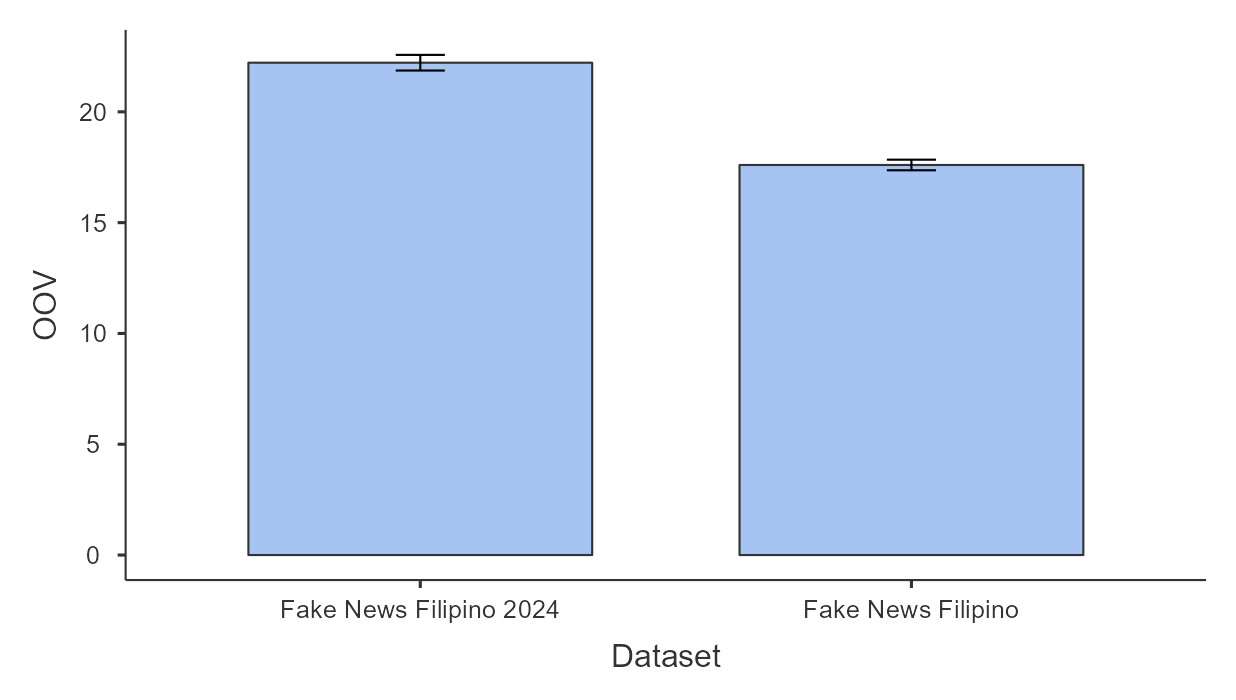
\includegraphics[width=\textwidth,height=\textheight, keepaspectratio]{figures/stats/oov_data.png}
        \caption{Bar plot of average OOV word count of Fake News Filipino and Fake News Filipino 2024.}
        \label{fig:oov_data}
\end{figure}
\begin{figure}[h!]
    \centering
    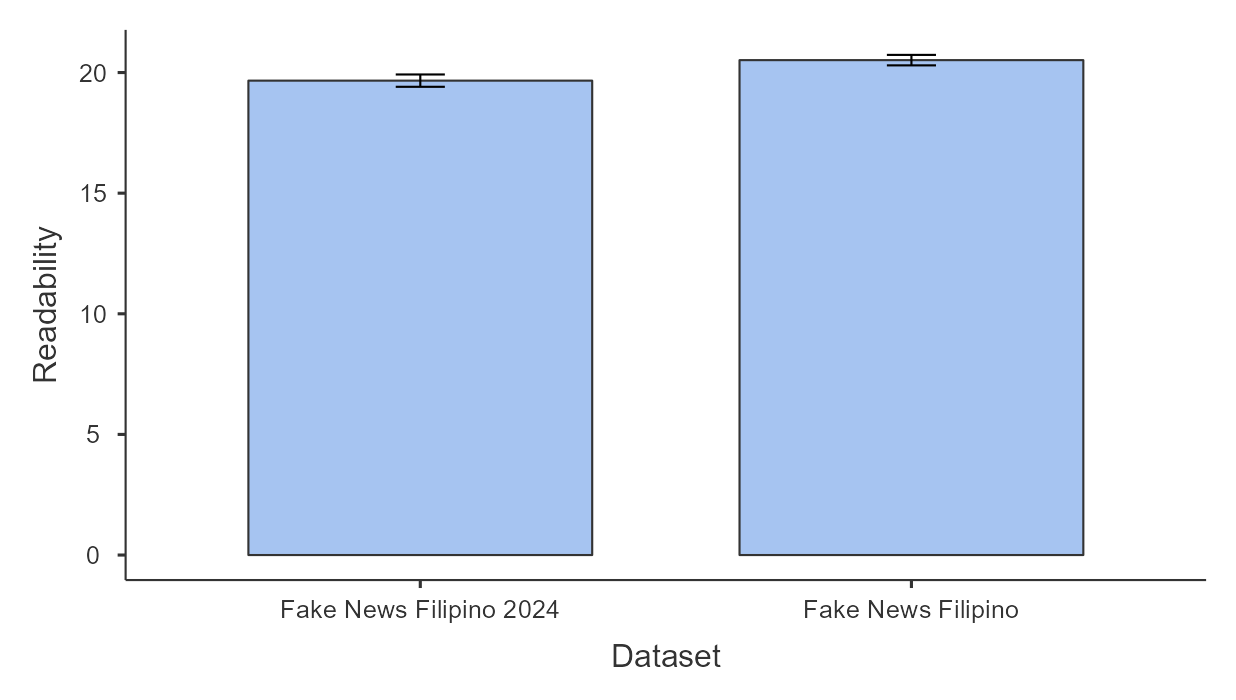
\includegraphics[width=\textwidth,height=\textheight, keepaspectratio]{figures/stats/read_data.png}
        \caption{Bar plot of average readability index of Fake News Filipino and Fake News Filipino 2024.}
        \label{fig:read_data}
\end{figure}
\begin{figure}[h!]
    \centering
    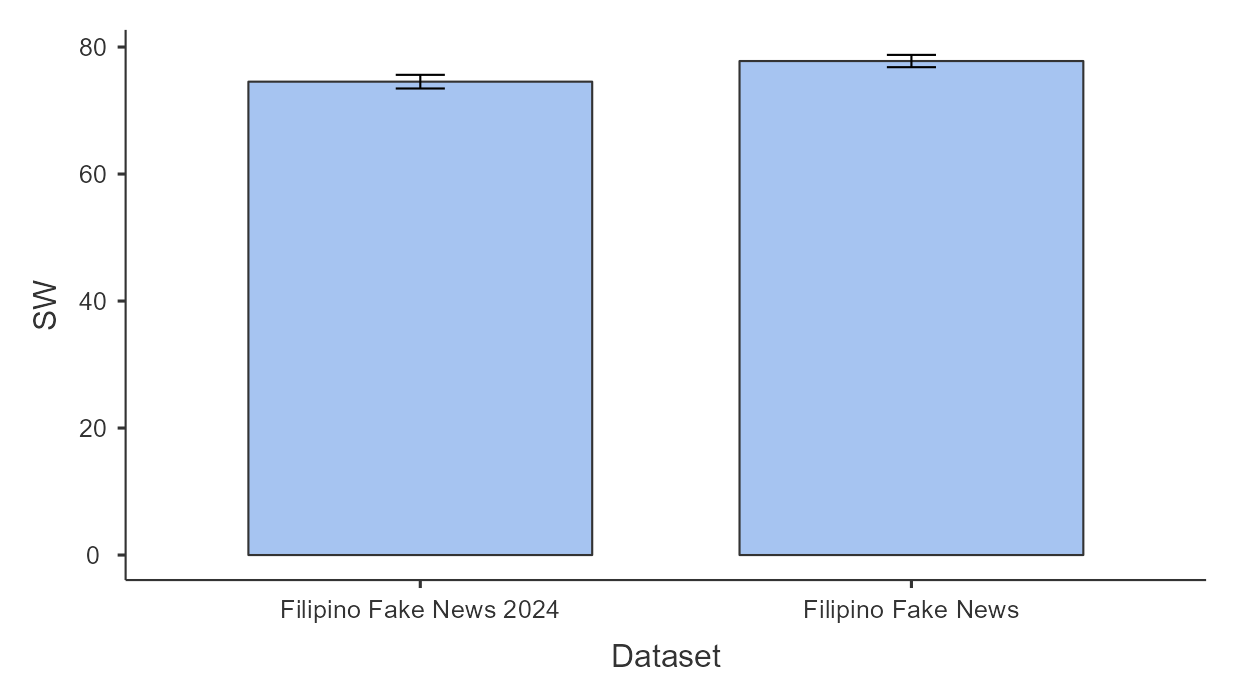
\includegraphics[width=\textwidth,height=\textheight, keepaspectratio]{figures/stats/sw_data.png}
        \caption{Bar plot of average stop word count Fake News Filipino and Fake News Filipino 2024.}
        \label{fig:sw_data}
\end{figure}

\section{Classifiers without Hyperparameter Tuning}

The models were trained on the combined dataset without hyperparameter tuning.

Figure \ref{MNB_default} shows the confusion matrix of \textbf{Multinomial Naive Bayes} without grid search. The model did not misclassify any instance of real news as fake news. However, it misclassified 537 instances of fake news as real news, significantly lowering its recall for fake news. It yielded an accuracy of approximately 0.58. It had the lowest recall for fake news at 0.16, signifying difficulty in identify true instances of fake news and a high false positive rate. The F1-score of real news and fake news were 0.70 and 0.28 respectively. These were relatively low scores.

\begin{figure}[h!]
    \centering
    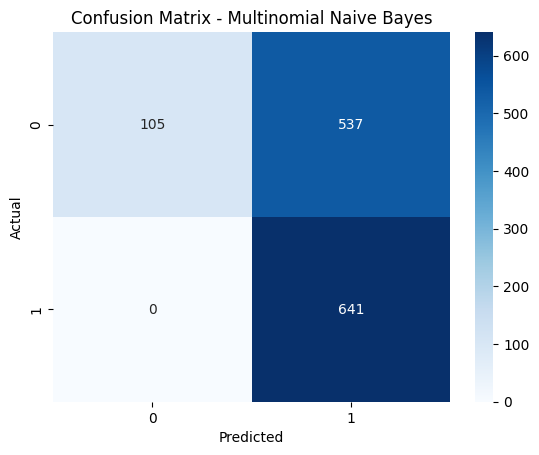
\includegraphics[width=0.6\textwidth,height=0.6\textheight, keepaspectratio]{figures/hyperparam/MNB_default.png}
        \caption{Confusion Matrix of Multinomial Naive Bayes without Grid Search.}
        \label{MNB_default}
\end{figure}

As shown in the confusion matrix of \textbf{Logistic Regression} at Figure \ref{LR_default}, the model misclassified 42 instances of fake news as real news and 51 instances of real news as fake news. It yielded an accuracy of approximately 0.93. It had a high recall for real news and fake news at both 0.93 and 0.92 respectively. The F1-scores for both real news and fake news were 0.93.

\begin{figure}[h!]
    \centering
    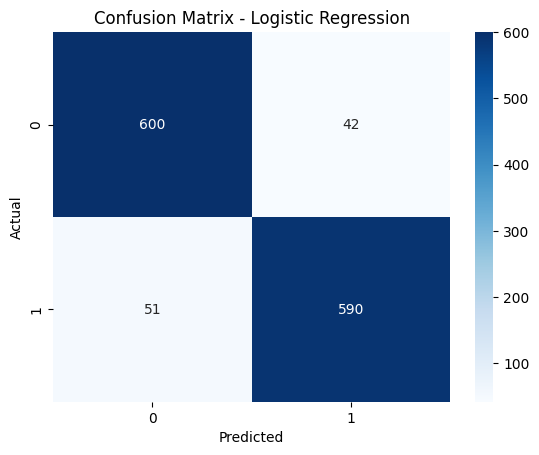
\includegraphics[width=0.6\textwidth,height=0.6\textheight, keepaspectratio]{figures/hyperparam/LR_default.png}
        \caption{Confusion Matrix of Logistic Regression without Grid Search.}
        \label{LR_default}
\end{figure}

Figure \ref{RF_default} depicts the confusion matrix of \textbf{Random Forest}. The model misclassified 66 instances of fake news and 59 instances of real news. It yielded an accuracy of approximately 0.90. It had a recall of 0.90 and 0.91 for fake news and real news respectively. The F1-score of both classes was 0.90, implying balanced metrics.

\begin{figure}[h!]
    \centering
    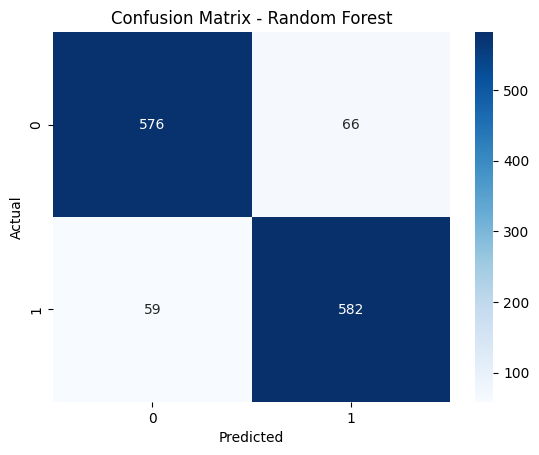
\includegraphics[width=0.6\textwidth,height=0.6\textheight, keepaspectratio]{figures/hyperparam/RF_default.png}
        \caption{Confusion Matrix of Multinomial Naive Bayes without Grid Search.}
        \label{RF_default}
\end{figure}

Based on Figure \ref{SVC_default}, \textbf{Support Vector Classifier}, misclassified 169 instances of fake news and 70 instances of real news. It had an accuracy of approximately 0.81. It had a relatively lower recall for fake news at 0.74. The F1-scores for real news and fake news were 0.80 and 0.83 respectively.

\begin{figure}[h!]
    \centering
    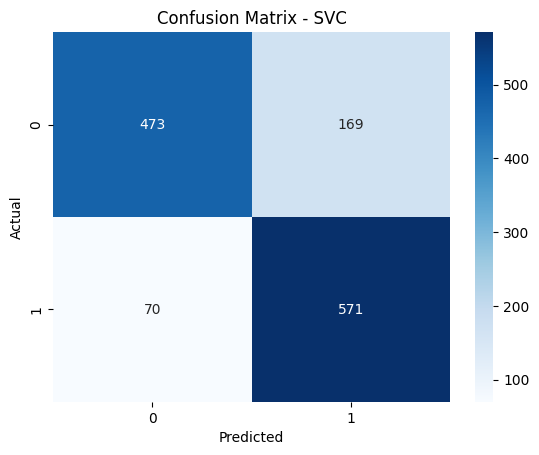
\includegraphics[width=0.6\textwidth,height=0.6\textheight, keepaspectratio]{figures/hyperparam/SVC_default.png}
        \caption{Confusion Matrix of Multinomial Naive Bayes without Grid Search.}
        \label{SVC_default}
\end{figure}

Results without hyperparameter tuning are summarized in Table \ref{tab:no_hyperparam_summary}. As shown in Table \ref{tab:no_hyperparam_summary}, Logistic Regression had the highest F1-scores while Multinomial Naive Bayes scored the lowest.

\begin{table}[ht]
    \centering
    \begin{tabular}{|l|ccc|ccc|}
    \hline
    & \multicolumn{3}{c|}{Multinomial Naive Bayes} & \multicolumn{3}{c|}{Logistic Regression} \\
    \hline
    & Precision & Recall & F1-score & Precision & Recall & F1-score \\
    \hline
    Fake & 1.00 & 0.16 & 0.28 & 0.92 & 0.93 & 0.93 \\
    Not Fake & 0.54 & 1.00 & 0.70 & 0.93 & 0.92 & 0.93 \\
    Accuracy & & & 0.58 & & & 0.93 \\
    \hline
    & \multicolumn{3}{c|}{Random Forest} & \multicolumn{3}{c|}{Support Vector Classifier} \\
    \hline
    & Precision & Recall & F1-score & Precision & Recall & F1-score \\
    \hline
    Fake & 0.91 & 0.90 & 0.90 & 0.87 & 0.74 & 0.80 \\
    Not Fake & 0.90 & 0.91 & 0.90 & 0.77 & 0.89 & 0.83 \\
    Accuracy & & & 0.90 & & & 0.81 \\
    \hline
    \end{tabular}
    \caption{Performance metrics for classifiers without hyperparameter tuning.}
    \label{tab:no_hyperparam_summary}
\end{table}



\section{Classifiers with Hyperparameter Tuning}
\label{sec:ParamTuning}
To the determine the optimal hyperparameters, all models were trained and tested on the combined dataset using grid search with five-fold cross validation.

Figure \ref{MNB_hyperparam} shows the performance of \textbf{Multinomial Naive Bayes} with an alpha of 0.01, the optimal hyperparameter based on the cross validation. The model misclassified 155 instances of fake news and 18 instances of real news. It yielded an accuracy of approximately 0.865. It had the lowest recall for fake news at 0.87.

\begin{figure}[h!]
\centering
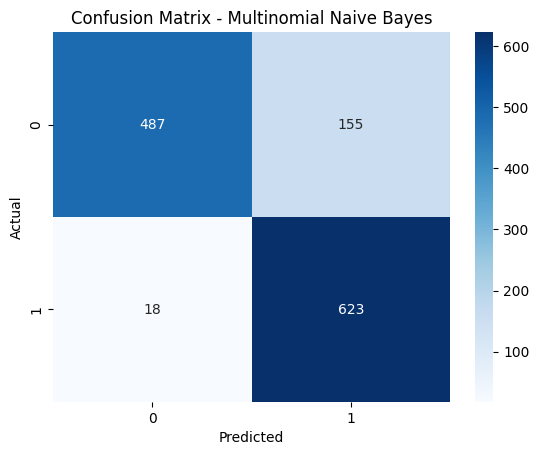
\includegraphics[width=0.6\textwidth,height=0.6\textheight, keepaspectratio]{figures/hyperparam/MNB.png}
    \caption{Confusion Matrix of Multinomial Naive Bayes with alpha = 0.01.}
    \label{MNB_hyperparam}
\end{figure}

The best hyperparameter for \textbf{Logistic Regression} was max\_iter = 2000. As shown in Figure \ref{LR_hyperparam}, Logistic Regression misclassified 42 instances of fake news and 51 instances of real news. It yielded an accuracy of 0.928 and an F1-score of 0.93 for both real news and fake news.

\begin{figure}[h!]
\centering
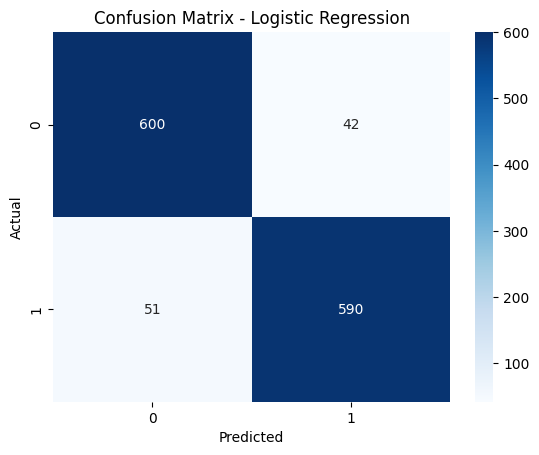
\includegraphics[width=0.6\textwidth,height=0.6\textheight, keepaspectratio]{figures/hyperparam/LR.png}
    \caption{Confusion Matrix of Linear Regression with max\_iter = 2000.}
    \label{LR_hyperparam}
\end{figure}

For \textbf{Random Forest}, max\_depth = 20 was the optimal hyperparameter. The performance of Random Forest is shown in Figure \ref{RF_hyperparam}. The model misclassified 80 instances of fake news and 63 instances of real news. It yielded an accuracy of 0.889 with an F1-score of 0.89 for both fake news and real news.

\begin{figure}[h!]
\centering
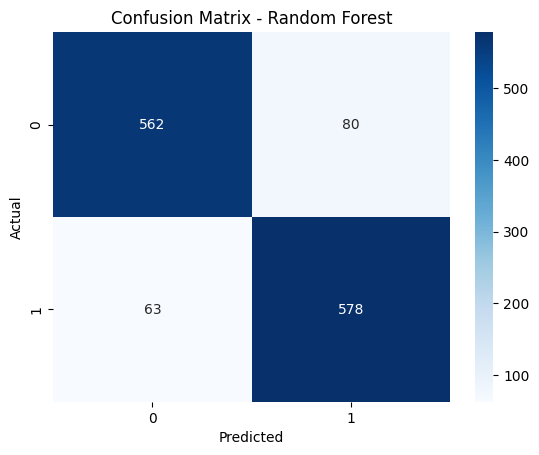
\includegraphics[width=0.6\textwidth,height=0.6\textheight, keepaspectratio]{figures/hyperparam/RF.png}
    \caption{Confusion Matrix of Random Forest with max\_depth = 20.}
    \label{RF_hyperparam}
\end{figure}

For \textbf{Support Vector Classifier}, the optimal hyperparameter was C = 0.1 with a linear kernel. As shown in Figure \ref{SVC_hyperparam}, the model misclassified 42 instances of fake news and 51 instances of real news. It yielded an accuracy of 0.928 and an F1-score of 0.93 for both fake news and real news.

Both Support Vector Classifier and Logistic Regression yielded the highest accuracy with hyperparameter tuning.

\begin{figure}[h!]
\centering
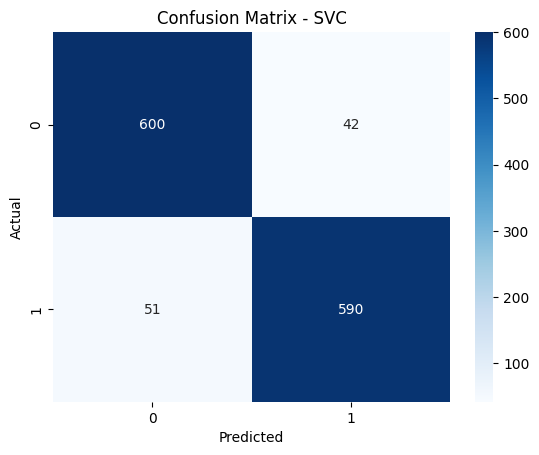
\includegraphics[width=0.6\textwidth,height=0.6\textheight, keepaspectratio]{figures/hyperparam/SVC.png}
    \caption{Confusion Support Vector Classifier with a linear kernel and C = 0.1.}
    \label{SVC_hyperparam}
\end{figure}

The results are summarized in Table \ref{tab:hyperparam_summary}. Both Logistic Regression and Support Vector Classifier scored the highest F1-scores while Random Forest scored the lowest. Comparing the accuracies of the classifiers without hyperparameter tuning in Table \ref{tab:no_hyperparam_summary} and their accuracies with hyperparameter tuning in Table \ref{tab:hyperparam_summary}, hyperparameter tuning significantly increased the accuracy of Multinomial Naive Bayes and Support Vector Classifier. However, hyperparameter tuning did not have any significant impact on the accuracies of Logistic Regression and Random Forest.

\begin{table}[ht]
    \centering
    \begin{tabular}{|l|ccc|ccc|}
    \hline
    & \multicolumn{3}{c|}{Multinomial Naive Bayes} & \multicolumn{3}{c|}{Logistic Regression} \\
    \hline
    & Precision & Recall & F1-score & Precision & Recall & F1-score \\
    \hline
    Fake & 0.93 & 0.76 & 0.85 & 0.92 & 0.93 & 0.93 \\
    Not Fake & 0.80 & 0.97 & 0.88 & 0.93 & 0.92 & 0.93 \\
    Accuracy & & & 0.87 & & & 0.93 \\
    \hline
    & \multicolumn{3}{c|}{Random Forest} & \multicolumn{3}{c|}{Support Vector Classifier} \\
    \hline
    & Precision & Recall & F1-score & Precision & Recall & F1-score \\
    \hline
    Fake & 0.90 & 0.88 & 0.89 & 0.92 & 0.93 & 0.93 \\
    Not Fake & 0.88 & 0.90 & 0.89 & 0.93 & 0.92 & 0.93 \\
    Accuracy & & & 0.89 & & & 0.93 \\
    \hline
    \end{tabular}
    \caption{Performance metrics for classifiers with hyperparameter tuning.}
    \label{tab:hyperparam_summary}
\end{table}

\section{Accuracy Testing}

Using the optimal hyperparameters in Section \ref{sec:ParamTuning}, all four models were trained and tested using five-fold cross validation six times, a total of 30 tests, across three datasets: Fake News Filipino (2020), Fake News Filipino 2024 (2024), and the combined corpus with the two datasets. Average accuracies of the models are shown in Table \ref{tab::AverageAccuracies}. Logistic Regression and Support Vector Classifier scored the highest average accuracy in both Fake News Filipino and Fake News Filipino 2024. But for the combined dataset, only Logistic Regression yielded the highest average accuracy. Compared to the other models across the three datasets, Multinomial Naive Bayes and Random Forest performed relatively worst in the combined dataset with accuracies of 86.0\% and 88.8\% respectively. Table \ref{tab::AverageAccuracies} shows the average accuracies of the models. The box plot of the accuracies is depicted in Figure \ref{fig:box_plot_accuracy}.

\singlespacing
\begin{tabularx}{\textwidth}{|l|l|c|}
    \hline Classifier & Dataset & Average Accuracy \\ \hline
    \endfirsthead

    \hline
    \multicolumn{3}{|r|}
    {Continued from previous page.} \\
    \hline
    Classifier & Dataset & Average Accuracy \\ \hline
    \endhead

    \hline \multicolumn{3}{|r|}{{Continued on next page...}} \\ \hline
    \endfoot

    \hline
    \caption{Average Accuracies of classifiers for each dataset.}
    \endlastfoot

    Logistic Regression & Fake News Filipino & 0.951 \\
    \cline{2-3}
    & Fake News Filipino 2024 & 0.947\\
    \cline{2-3}
    & Combined & 0.924 \\
    \hline
    Multinomial Naive Bayes & Fake News Filipino & 0.923 \\
    \cline{2-3}
    & Fake News Filipino 2024 & 0.885 \\
    \cline{2-3}
    & Combined & 0.860 \\
    \hline
    Random Forest & Fake News Filipino & 0.919 \\
    \cline{2-3}
    & Fake News Filipino 2024 & 0.926 \\
    \cline{2-3}
    & Combined & 0.888 \\
    \hline
    Support Vector Classifier & Fake News Filipino & 0.951 \\
    \cline{2-3}
    & Fake News Filipino 2024 & 0.947 \\
    \cline{2-3}
    & Combined & 0.922
\label{tab::AverageAccuracies}
\end{tabularx}
\doublespacing

\begin{figure}[h!]
    \centering
    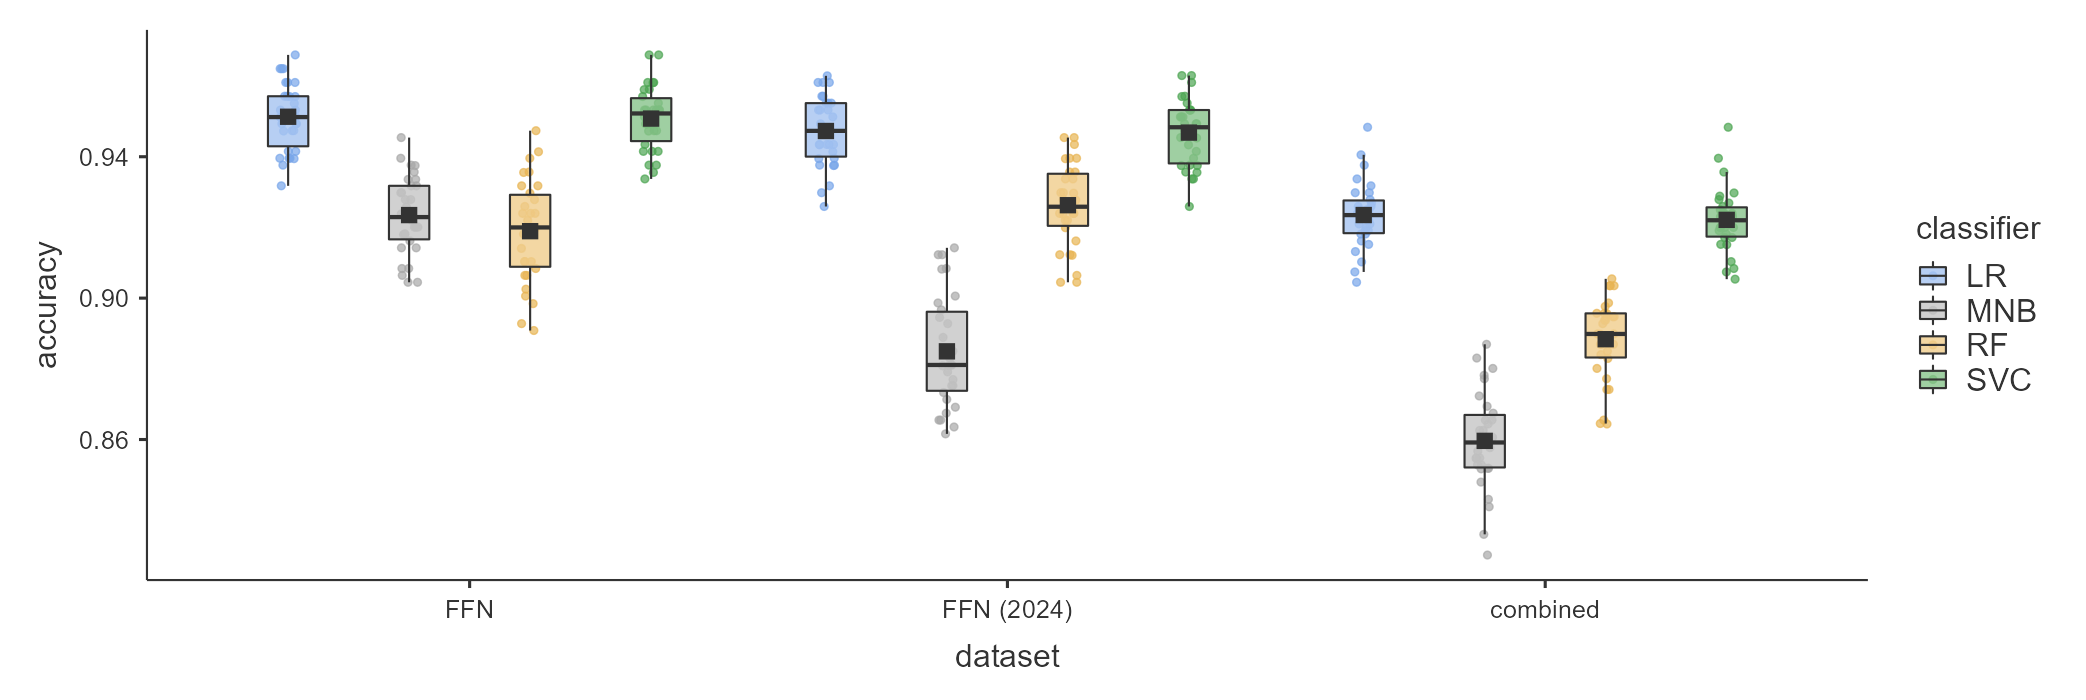
\includegraphics[width=\textwidth,height=\textheight, keepaspectratio]{figures/stats/box_plot.png}
        \caption{Box plot of the accuracies accross datasets.}
        \label{fig:box_plot_accuracy}
\end{figure}

The Shapiro-Wilk test was used to assess the normality of each group in a two-way format, where accuracies were the dependent variable, and datasets and classifiers were the factors. As shown in Table \ref{tab::normality_tests}, all groups have \textit{p}-values greater than or equal to 0.05 indicating that the data is normally distributed in the two-way format. However, with a \textit{p}-value (0.003) lower than 0.05, Levene's test determined the variances of the groups to be heterogenous.

\singlespacing
\begin{tabularx}{\textwidth}{|l|l|l|l|}
    \hline
    Dataset & Classifier & Statistic & \textit{p}-value \\
    \hline
    Fake News Filipino & LR & 0.968 & 0.492 \\
    \cline{2-4}
    & MNB & 0.971 & 0.571 \\
    \cline{2-4}
    & RF & 0.985 & 0.938 \\
    \cline{2-4}
    & SVC & 0.972 & 0.603 \\
    \hline
    Fake News Filipino 2024 & LR & 0.963 & 0.363 \\
    \cline{2-4}
    & MNB & 0.940 & 0.928 \\
    \cline{2-4}
    & RF & 0.962 & 0.342 \\
    \cline{2-4}
    & SVC & 0.972 & 0.598 \\
    \hline
    Combined & LR & 0.979 & 0.793 \\
    \cline{2-4}
    & MNB & 0.981 & 0.852 \\
    \cline{2-4}
    & RF & 0.934 & 0.063 \\
    \cline{2-4}
    & SVC & 0.950 & 0.164 \\
    \hline
\caption{Shapiro-Wilk normality test in a two-way format.}
\label{tab::normality_tests}
\end{tabularx}
\doublespacing

To determine if there were significant differences between accuracies of different classifiers in different datasets, and taking into account the heteroscedacity of the data, two-way ANOVA for trimmed means was performed. As shown in Table \ref{tab::two-way} there was a significant difference (\textit{p}-value = 0.001) between accuracies in different datasets averaged across the classifiers. Additionally, there was a significant difference (\textit{p}-value = 0.001) between accuracies in the classifiers averaged across the datasets. Furthermore, their interaction effect was also significant (\textit{p}-value = 0.001). Thus, accuracy was affected both by the main effects of the dataset and classifier and also their combinations.

\begin{tabularx}{\textwidth}{|l|l|l|}
    \hline
    Factor & Statistic & \textit{p}-value \\
    \hline
    dataset & 689.45 & 0.001 \\
    \hline
    classifier & 1010.0371 & 0.001 \\
    \hline
    dataset*classifier & 129.07 & 0.001 \\
    \hline
\caption{Two-way ANOVA for Trimmed Means.}
\label{tab::two-way}
\end{tabularx}

To determine which classifiers had significant differences within the different datsets, post-hoc mean-separation testing was conducted using Bonferroni Correction for subgroups of each dataset level. As shown in Table \ref{tab::post-hoc-dataset-lvl}, the only subgroups that did not have significant differences were Logistic Regression and Support Vector Classifier across all datasets, as well as Multinomial Naive Bayes and Random Forest in the Fake News Filipino dataset.

The results were reflected in the interaction plot of the accuracies in Figure \ref{fig:interaction_plot}. As shown in Figure \ref{fig:interaction_plot}, the accuracies of Logistic Regression and Support Vector Classifier were almost equal across all datasets. The same could be said for the accuracy of Multinomial Naive Bayes and Random Forest in the Fake News Filipino dataset. It could also be observed that the performance of the classifiers changes depending on the dataset just as the two-way ANOVA suggested.

To determine which classifiers had significant differences between datasets, a similar post-hoc test was conducted for subgroups of each classifier level. Table \ref{tab::post-hoc-classifier-lvl} shows that only Multinomial Naive Bayes had a significant change in performance between Fake News Filipino 2024 and Fake News Filipino dataset. Furthermore, all accuracies of the classifiers differ significantly in the combined dataset compared with their accuracies in either Fake News Filipino or Fake News Filipino 2024.

\begin{figure}[h!]
    \centering
    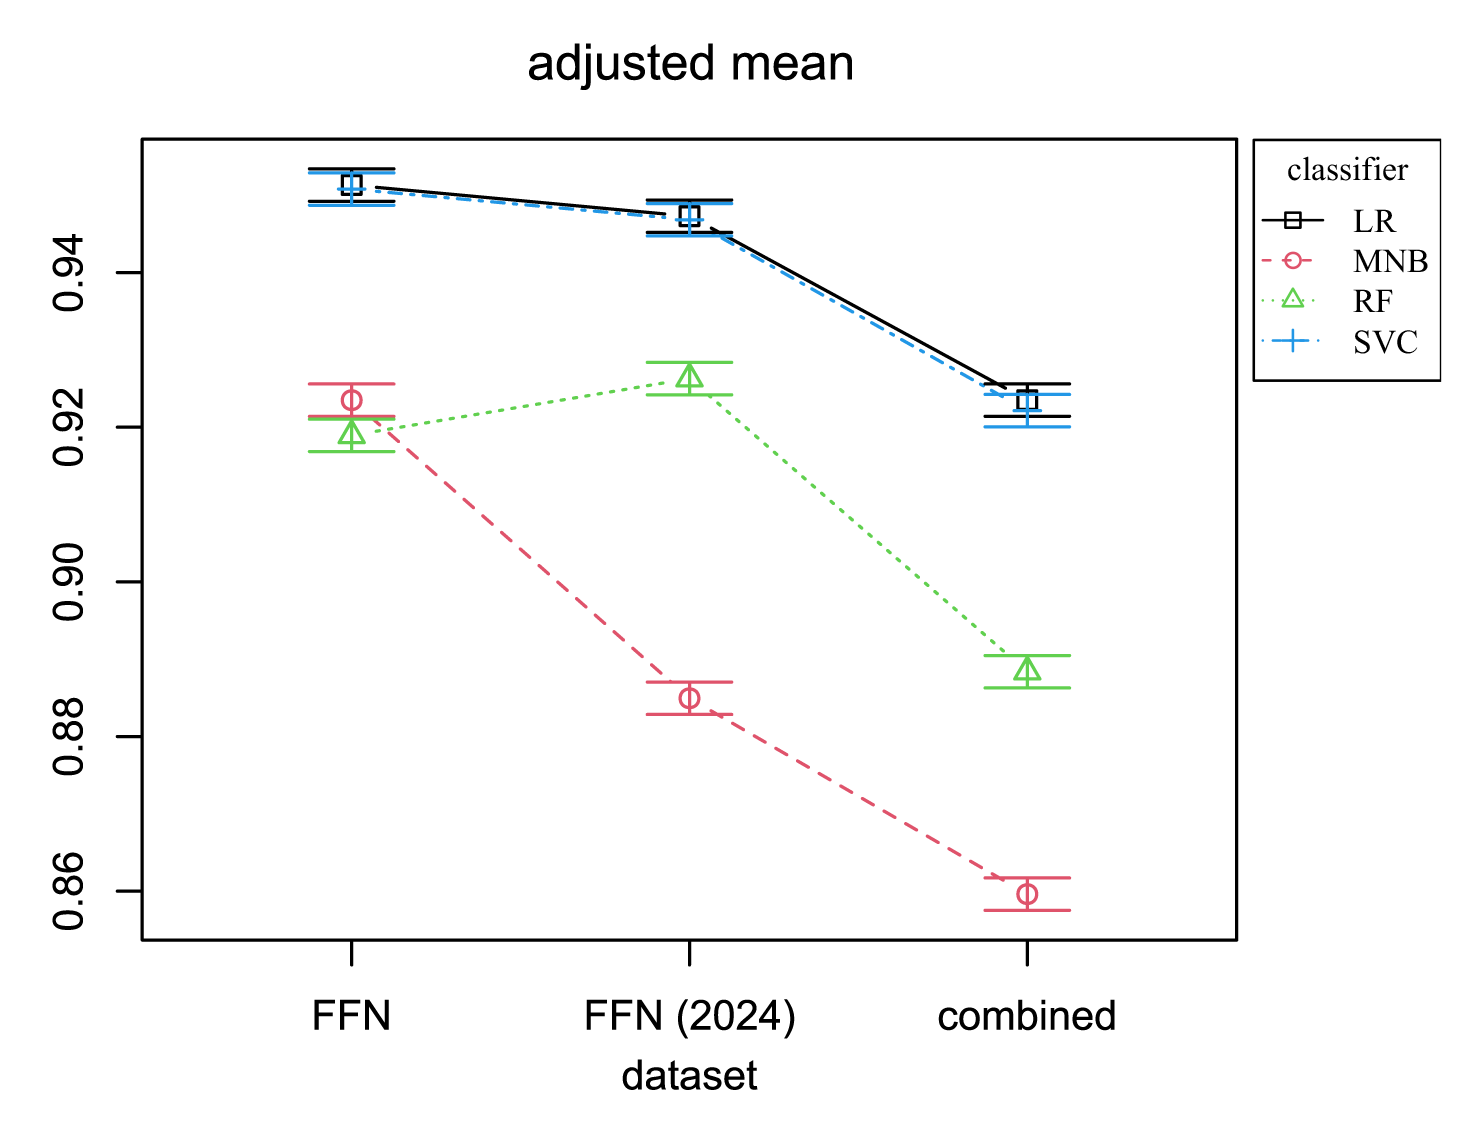
\includegraphics[width=\textwidth,height=\textheight, keepaspectratio]{figures/stats/im.png}
        \caption{Interaction plot of accuracies across datasets.}
        \label{fig:interaction_plot}
\end{figure}

\singlespacing
\begin{tabularx}{\textwidth}{|l|l|l|l|}
    \hline Dataset & Classifier (a) & Classifier(b) & \textit{p}-value \\ \hline
    \endfirsthead

    \hline
    \multicolumn{4}{|r|}
    {Continued from previous page.} \\

    \hline
    Dataset & Classifier (a) & Classifier(b) & \textit{p}-value \\ \hline
    \endhead

    \hline \multicolumn{4}{|r|}{{Continued on next page...}} \\ \hline
    \endfoot

    \hline
    \caption{Bonferroni correction for subgroups of each dataset level.}
    \endlastfoot

    Fake News Filipino & LR & MNB & \textless 0.001 \\
    \cline{3-4}
    & & RF & \textless 0.001 \\
    \cline{3-4}
    & & SVC & 1.00 \\
    \cline{2-4}
    & MNB & RF & 1.00 \\
    \cline{3-4}
    & & SVC & \textless 0.001 \\
    \cline{2-4}
    & RF & SVC & \textless 0.001 \\
    \hline
    Fake News Filipino 2024 & LR & MNB & \textless 0.001 \\
    \cline{3-4}
    & & RF & \textless 0.001 \\
    \cline{3-4}
    & & SVC & 1.00 \\
    \cline{2-4}
    & MNB & RF & \textless 0.001 \\
    \cline{3-4}
    & & SVC & \textless 0.001 \\
    \cline{2-4}
    & RF & SVC & \textless 0.001 \\
    \hline
    Combined & LR & MNB & \textless 0.001 \\
    \cline{3-4}
    & & RF & \textless 0.001 \\
    \cline{3-4}
    & & SVC & 1.00 \\
    \cline{2-4}
    & MNB & RF & \textless 0.001 \\
    \cline{3-4}
    & & SVC & \textless 0.001 \\
    \cline{2-4}
    & RF & SVC & \textless 0.001
\label{tab::post-hoc-dataset-lvl}
\end{tabularx}
\doublespacing

\singlespacing
\begin{tabularx}{\textwidth}{|l|l|l|l|}
    \hline Classifier & Dataset(a) & Dataset(b) & \textit{p}-value \\ \hline
    \endfirsthead

    \hline
    \multicolumn{4}{|r|}
    {Continued from previous page.} \\

    \hline
    Classifier & Dataset(a) & Dataset(b) & \textit{p}-value \\ \hline
    \endhead

    \hline \multicolumn{4}{|r|}{{Continued on next page...}} \\ \hline
    \endfoot

    \hline
    \caption{Bonferroni correction for subgroups of each classifier level.}
    \endlastfoot

    LR & Fake News Filipino & Fake News Filipino 2024 & 0.485 \\
    \cline{3-4}
    & & Combined & \textless 0.001 \\
    \cline{2-4}
    & Fake News Filipino 2024 & Combined & \textless 0.001 \\
    \hline
    MNB & Fake News Filipino & Fake News Filipino 2024 & \textless 0.001 \\
    \cline{3-4}
    & & Combined & \textless 0.001 \\
    \cline{2-4}
    & Fake News Filipino 2024 & Combined & \textless 0.001 \\
    \hline
    RF & Fake News Filipino & Fake News Filipino 2024 & 0.150 \\
    \cline{3-4}
    & & Combined & \textless 0.001 \\
    \cline{2-4}
    & Fake News Filipino 2024 & Combined & \textless 0.001 \\
    \hline
    SVC & Fake News Filipino & Fake News Filipino 2024 & 0.421 \\
    \cline{3-4}
    & & Combined & \textless 0.001 \\
    \cline{2-4}
    & Fake News Filipino 2024 & Combined & \textless 0.001
\label{tab::post-hoc-classifier-lvl}
\end{tabularx}
\doublespacing

\pagebreak
\section{Application Testing}
The FaKe web extension was assessed using three prominent browsers: Google Chrome, Microsoft Edge, and Mozilla Firefox. As of 2023,
Google Chrome, Safari, Microsoft Edge, and Mozilla Firefox rank among the most popular internet browsers with 63.56\%, 19.84\%,
5.43\%, and 2.95\%  market shares respectively \cite{statista2024}. Windows is the most widely used operating system, followed by
MacOS and Linux \cite{idris2021}. Apple devices were unavailable, limiting the assessment of cross-platform compatibility.
Moreover, Apple Safari no longer offered Safari updates for Windows devices, with the 2010 version of Safari being the last
version created for Windows \cite{apple2024}. Due to this, Apple Safari was not chosen as a test browser. The evaluation utilized identical articles categorized as fake news or real news. Figures \ref{fig:fake-chrome-test} and \ref{fig:real-chrome-test} display the outcomes using Google Chrome. Figures \ref{fig:fake-edge-test} and \ref{fig:real-edge-test} display the outcomes for Microsoft Edge. Lastly, Figures \ref{fig:fake-firefox-test} and \ref{fig:real-firefox-test} display the outcomes for Mozilla Firefox. The results demonstrate that the application's functionality remained uniform across different browsers.

        \begin{figure}[h!]
            \centering
            
\includegraphics[width=1\textwidth,height=1\textheight, keepaspectratio]{figures/Screenshots/chrome-true-positive.png}
            \caption{FaKe Extension testing with Google Chrome (Real).}
            \label{fig:real-chrome-test}
        \end{figure}

        \begin{figure}[h!]
            \centering
            
\includegraphics[width=1\textwidth,height=1\textheight, keepaspectratio]{figures/Screenshots/chrome-true-negative.png}
            \caption{FaKe Extension testing with Google Chrome (Fake).}
            \label{fig:fake-chrome-test}
            \end{figure}

        \begin{figure}[h!]
            \centering
            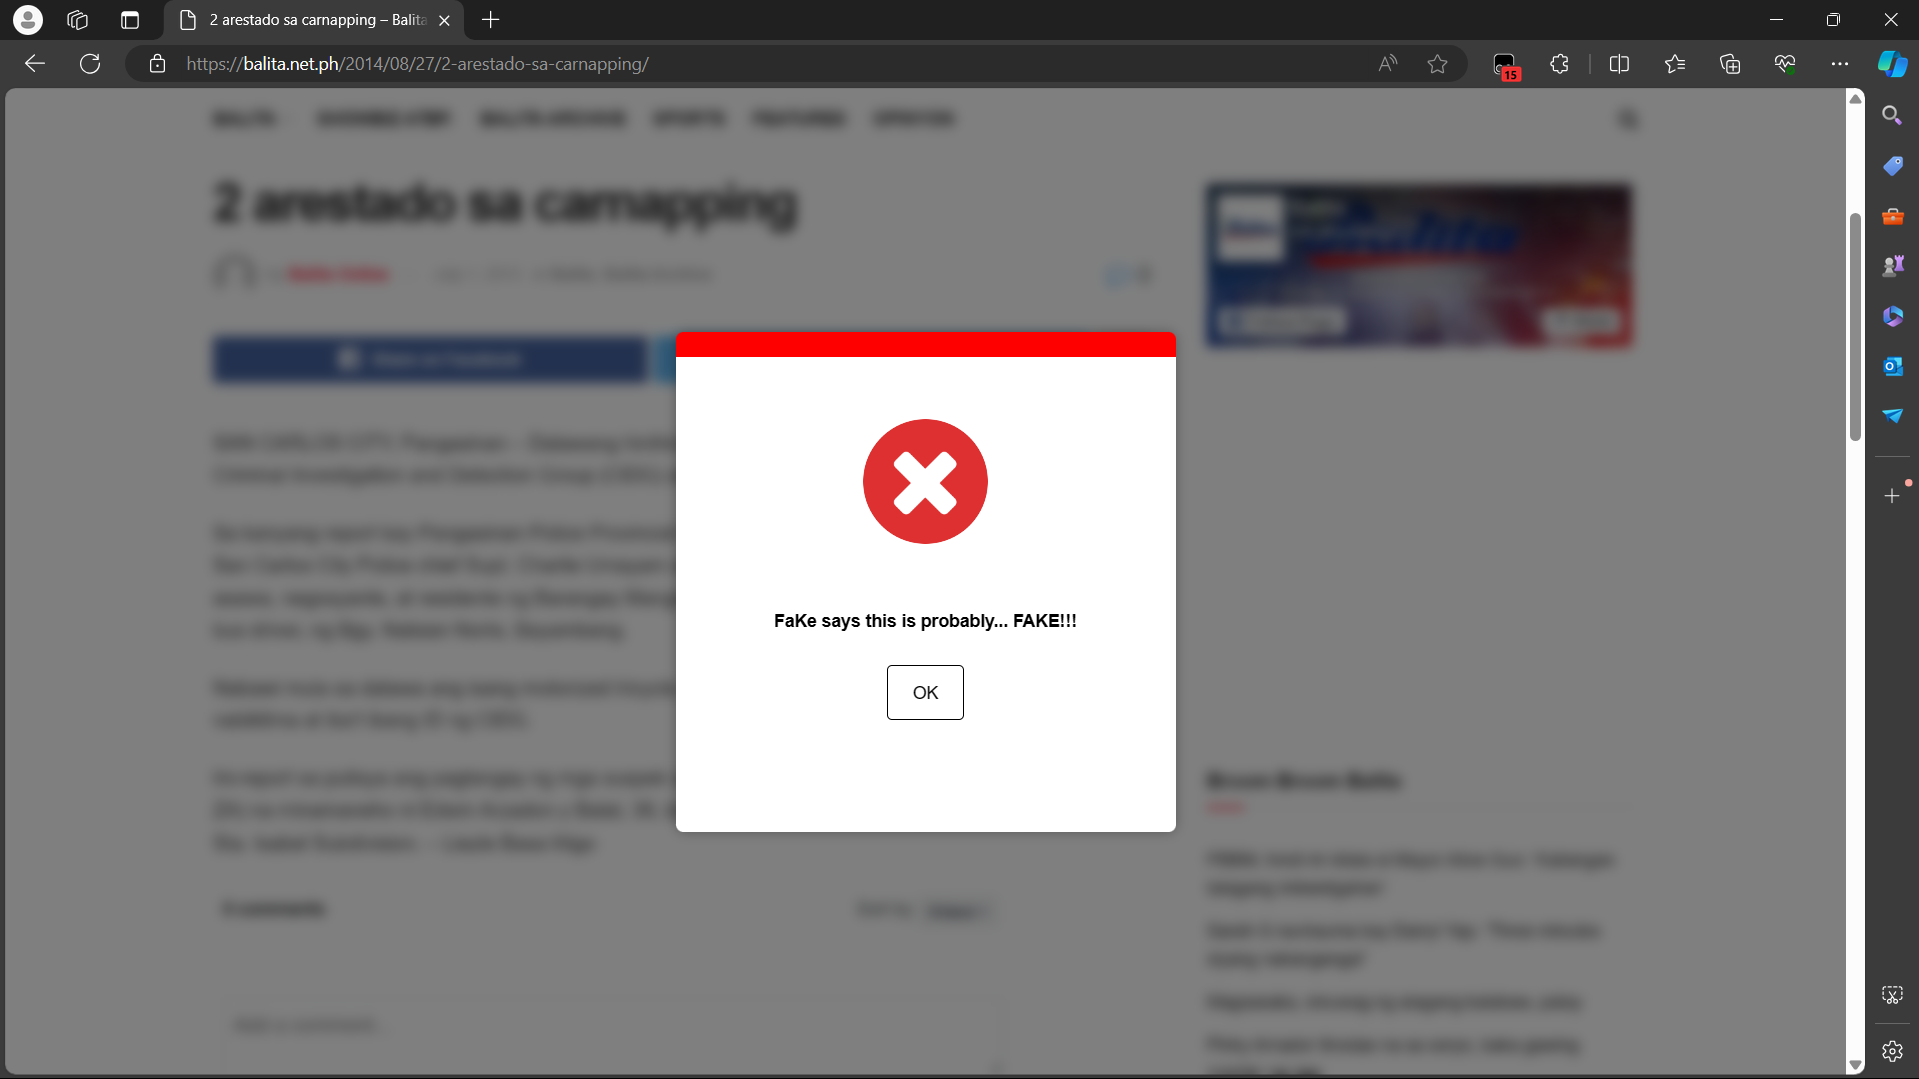
\includegraphics[width=1\textwidth,height=1\textheight, keepaspectratio]{figures/Screenshots/edge-true-positive.png}
            \caption{FaKe Extension testing with Microsoft Edge (Real).}
            \label{fig:real-edge-test}
        \end{figure}

        \begin{figure}[h!]
            \centering
            
\includegraphics[width=1\textwidth,height=1\textheight, keepaspectratio]{figures/Screenshots/edge-true-negative.png}
            \caption{FaKe Extension testing with Microsoft Edge (Fake).}
            \label{fig:fake-edge-test}
        \end{figure}

        \begin{figure}[h!]
            \centering
            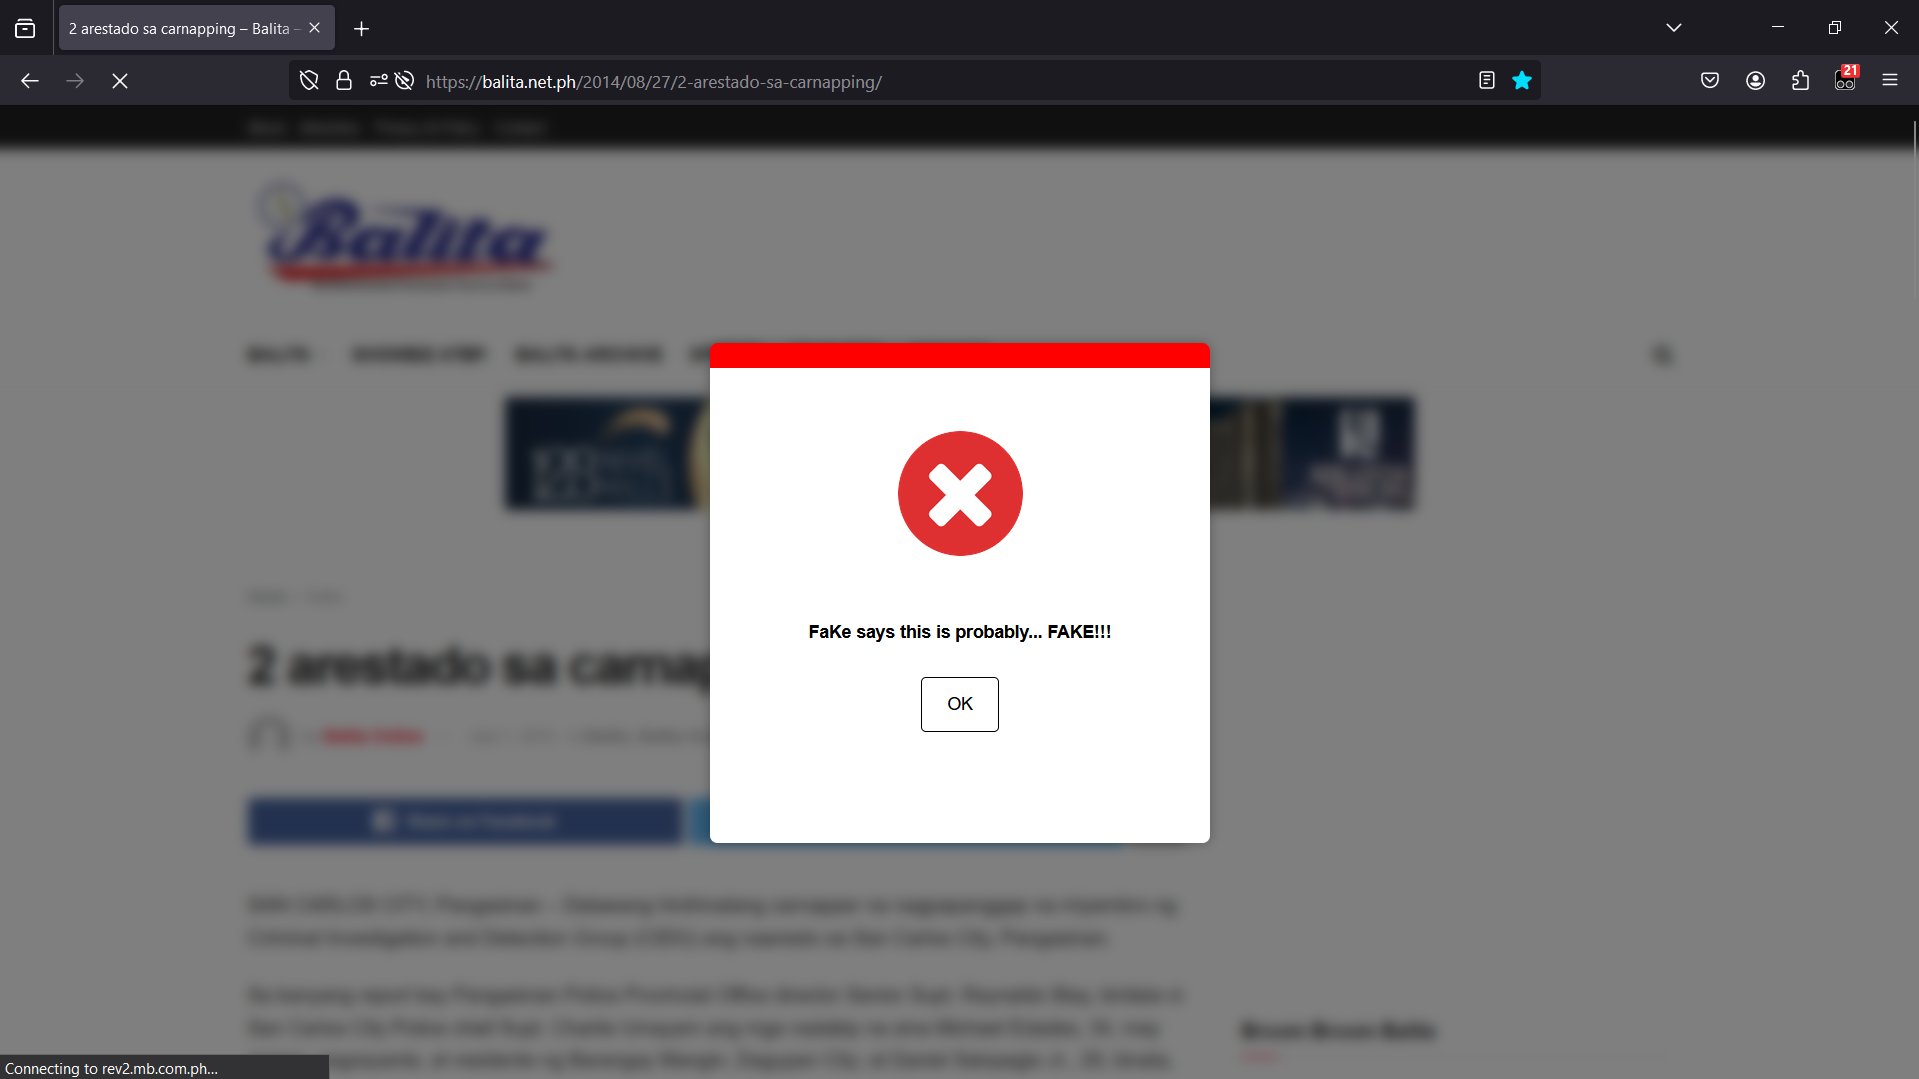
\includegraphics[width=1\textwidth,height=1\textheight, keepaspectratio]{figures/Screenshots/firefox-true-positive.png}
            \caption{FaKe Extension testing with Mozilla Firefox (Real).}
            \label{fig:real-firefox-test}
        \end{figure}

        \begin{figure}[h!]
            \centering
            
\includegraphics[width=1\textwidth,height=1\textheight, keepaspectratio]{figures/Screenshots/firefox-true-negative.png}
            \caption{FaKe Extension testing with Mozilla Firefox (Fake).}
            \label{fig:fake-firefox-test}
        \end{figure}

        Figures \ref{fig:false-positive-news-article}, \ref{fig:true-positive-news-article}, \ref{fig:false-negative-news-article}, and \ref{fig:true-negative-news-article} show sample articles, the predictions that the classifier makes on them (classifier label), and their actual categories (gold label). These articles were not included in the joint corpus used during training.

                \begin{figure}[h!]
                    \centering
                    \fbox{%
                    \parbox{\textwidth}{% TODO Translate the text properly Italicize the translation
                    \small \raggedright Mahaharap sa kasong administratibo ang isang opisyal ng pulisya matapos magwala sa mismong himpilan, pinasok sa opisina ang kanyang hepe at pinagsasalitaan umano ng masama, Lunes ng gabi, sa Bacoor City, Cavite.\linebreak

                    \small \raggedright Kasong grave misconduct ang kakaharapin ni Chief Insp. Virgilio Rubio, deputy chief ng Bacoor City Police, batay sa reklamo ni Supt. Rommel Estolano.\linebreak

                    \small \raggedright Sa ulat sa tanggapan ni Cavite Police Provincial Office director Senior Supt. Joselito Esquivel, bandang 7:30 ng gabi nang magtungo sa istasyon ng pulisya si Rubio na lasing na lasing, biglang pinaghahagis ang mga upuan at iba pang gamit sa opisina hanggang pumasok sa tanggapan ni Rubio habang may hawak na baril at nagbitiw ng kung anu-anong masasamang salita.\linebreak

                    \small \raggedright Gayunman, naawat ni Senior Insp. Chey Chey Saulog si Rubio at pinalabas sa himpilan ng pulisya.\linebreak\linebreak
                      \noindent\rule{0.5\textwidth}{0.4pt}\linebreak\linebreak

                      Translation:\newline \newline
                      \small \raggedright A police officer will face administrative charges after he disappeared from the station, his boss entered the office and allegedly badmouthed him, Monday night, in Bacoor City, Cavite.\linebreak

                      \small \raggedright Chief Insp. Virgilio Rubio, deputy chief of the Bacoor City police, will face a case of grave misconduct based on the complaint of Supt. Rommel Estolano.\linebreak

                      \small \raggedright In a report to the office of Cavite Police Provincial Office director Senior Supt. Joselito Esquivel, around 7:30 in the evening when Rubio went to the police station who was very drunk, suddenly threw chairs and other items in the office until he entered Rubio's office with a gun in his hand and uttered various bad words.\linebreak

                      \small \raggedright However, Senior Insp. Chey Chey Saulog intervened and escorted Rubio out of the police station.\linebreak\linebreak

                      \textbf{Classifier Label: Real} \newline
                      \textbf{Gold Label: Fake}

                        }
                    }

                     \caption{False Positive News Article}
                        \label{fig:false-positive-news-article}
                    \end{figure}

                    \begin{figure}[h!]
                        \centering
                        \fbox{%
                        \parbox{\textwidth}{% TODO Translate the text properly Italicize the translation
                        \small \raggedright SAN CARLOS CITY, Pangasinan – Dalawang hinihinalang carnapper na nagpapanggap na miyembro ng Criminal Investigation and Detection Group (CIDG) ang naaresto sa San Carlos City, Pangasinan. \linebreak

                        \small \raggedright Sa kanyang report kay Pangasinan Police Provincial Office director Senior Supt. Reynaldo Biay, kinilala ni San Carlos City Police chief Supt. Charlie Umayam ang mga nadakip na sina Michael Edades, 34, may asawa, negosyante, at residente ng Barangay Mangin, Dagupan City; at Daniel Salopagio Jr., 29, binata, bus driver, ng Bgy. Nalsian Norte, Bayambang.\linebreak

                        \small \raggedright Nabawi mula sa dalawa ang isang motorized tricycle, isang Sony Ericsson cell phone ng kanilang nabiktima at iba’t ibang ID ng CIDG. \linebreak

                        \small \raggedright Ini-report sa pulisya ang pagtangay ng mga suspek sa isang Honda TMX 155 motorized tricycle (8150-ZA) na minamaneho ni Edwin Arzadon y Balat, 36, biyudo, ng lungsod, madaling araw noong Linggo sa Sta. Isabel Subdivision.\linebreak\linebreak
                          \noindent\rule{0.5\textwidth}{0.4pt}\linebreak\linebreak

                          Translation:\newline \newline
                          \small \raggedright A police officer will face administrative charges after he disappeared from the station, his boss entered the office and allegedly badmouthed him, Monday night, in Bacoor City, Cavite.\linebreak

                          \small \raggedright Chief Insp. Virgilio Rubio, deputy chief of the Bacoor City police, will face a case of grave misconduct based on the complaint of Supt. Rommel Estolano.\linebreak

                          \small \raggedright In a report to the office of Cavite Police Provincial Office director Senior Supt. Joselito Esquivel, around 7:30 in the evening when Rubio went to the police station who was very drunk, suddenly threw chairs and other items in the office until he entered Rubio's office with a gun in his hand and uttered various bad words.\linebreak

                          \small \raggedright However, Senior Insp. Chey Chey Saulog intervened and escorted Rubio out of the police station.\linebreak\linebreak

                          \textbf{Classifier Label: Fake} \newline
                          \textbf{Gold Label: Fake}

                            }
                        }

                         \caption{True Negative News Article}
                            \label{fig:true-positive-news-article}
                        \end{figure}

                        \begin{figure}[h!]
                            \centering
                            \fbox{%
                            \parbox{\textwidth}{% TODO Translate the text properly Italicize the translation
                            \small \raggedright \textbf{Binigyan ng tatlong taong extension para sa kanyang panunungkulan bilang Commissioner ng Philippine Basketball Association si Willie Marcial} \linebreak

                            \small \raggedright Sa kanilang annual planning session sa Star Hotels sa bansang Italya, gaya ng naging pagkakatalaga sa kanya bilang Commissioner ng liga, naging unanimous ang pagbibigay ng board of governors ng extension sa termino ni Marcial kahapon (Huwebes). \linebreak

                            \small \raggedright May nalalabi pang isang taon sa naunang tatlong taong kontrata na nilagdaan ni Marcial noong 2018 pero binigyan sya ng PBA board ng bagong vote of confidence.\linebreak

                            \small \raggedright Ito’y bunga na rin ng magandang performance nito na nagustuhan ng board.“We’re open and very transparent about his performance,” wika ni PBA Chairman Ricky Vargas tungkol kay Marcial.\linebreak

                            \small \raggedright
                            \noindent\rule{0.5\textwidth}{0.4pt}\linebreak\linebreak

                              Translation:\newline \newline

                              \small \raggedright \textbf{Willie Marcial was given a three year extension for his tenure as the Commissioner of the Philippine Basketball Association.}\linebreak

                              \small \raggedright In their annual planning session at Star Hotels in Italy, similar to his appointment as the Commissioner of the league, the board of governors unanimously agreed to extend Marcial's term yesterday (Thursday).  \linebreak

                              \small \raggedright Marcial still has one year remaining in the initial three-year contract he signed in 2018, but he was given a new vote of confidence by the PBA board.\linebreak

                              \small \raggedright This is the result of his good performance that the board liked. “We’re open and very transparent about his performance,” said by PBA Chairman Ricky Vargas about Marcial. \linebreak
                                \linebreak\linebreak

                                \textbf{Classifier Label: Fake} \newline
                                \textbf{Gold Label: Real}

                            }
                          }
                             \caption{False Negative News Article}
                                \label{fig:false-negative-news-article}
                            \end{figure}

                    \begin{figure}[h!]
                        \centering
                        \fbox{%
                        \parbox{\textwidth}{% TODO Translate the text properly Italicize the translation
                        \small \raggedright Patay ang isang 5-anyos na lalaki sa Lapu-Lapu City, Cebu matapos umano siyang pukpukin sa ulo at ihagis sa dagat ng kaniyang 14-anyos na kapatid.\linebreak

                        \small \raggedright Sa ulat ng ABS-CBN News, nangyari ang insidente sa Sitio Lawis, Barangay Suba-Basbas nitong Biyernes ng umaga, Mayo 10.\linebreak

                        \small \raggedright Naglalaro lamang daw ang dalawa nang bigla umanong kumuha ng bato ang 14-anyos at ipinukpok ito sa 5-anyos niyang kapatid.\linebreak

                        \small \raggedright Nang mawalan ng malay ang biktima ay doon na siya tinulak sa dagat ng hanggang sa malunod, ayon kay Police Lt. Col. Christian Torres.\linebreak

                        \small \raggedright Dagdag pa ng ulat, napag-alaman umano sa imbestigasyon ng pulisya na magkaiba ang ama ng magkapatid at galit umano ang 14-anyos sa tatay ng 5-anyos na biktima.\linebreak

                        \small \raggedright Dahil menor de edad ang suspek, isinailalim umano siya sa isang home care facility.\linebreak

                        \small \raggedright Patuloy pa rin namangnagsasagawa ang mga awtoridad ng imbestigasyon hinggil sa naturang insidente.\linebreak

                        \noindent\rule{0.5\textwidth}{0.4pt}\linebreak\linebreak

                          Translation:\newline \newline

                          \small \raggedright A 5-year-old boy died in Lapu-Lapu City, Cebu after he was allegedly hit on the head and thrown into the sea by his 14-year-old brother.\linebreak

                          \small \raggedright According to ABS-CBN News, the incident happened in Sitio Lawis, Barangay Suba-Basbas this Friday morning, May 10.\linebreak

                          \small \raggedright It is said that the two were just playing when the 14-year-old suddenly took a rock and hit his 5-year-old brother with it.\linebreak

                          \small \raggedright When the victim lost consciousness, he was then pushed into the sea until he drowned, according to Police Lt. Col. Christian Torres.\linebreak

                          \small \raggedright The report added that the police investigation revealed that the brothers' fathers were different and that the 14-year-old was angry with the father of the 5-year-old victim.\linebreak

                          \small \raggedright Because the suspect is a minor, he was allegedly placed under a home care facility.\linebreak

                          \small \raggedright Authorities are still investigating the incident.\linebreak
                            \linebreak\linebreak

                            \textbf{Classifier Label: Real} \newline
                            \textbf{Gold Label: Real}

                        }
                      }
                         \caption{True Positive News Article}
                            \label{fig:true-negative-news-article}
                        \end{figure}
\clearpage
\pagebreak
\section{Summary} \label{dataset-limitation}

As shown in the results of two-way ANOVA together with the post-hoc tests, three out of four classifiers, namely Logistic Regression, Random Forest, and Support Vector Classifier, did not exhibit a significant change in performance between Fake News Filipino and Fake News Filipino 2024. However, the accuracies of all classifiers were significantly lower on the joint corpus. The reason for this may be attributed to differences in the writing styles of the news articles found between the two datasets. This is supported by the differences in the number of out-of-vocabulary words, the number of stop words, and the readability scores of the two datasets. This means that when the classifiers were trained on the two datasets separately, they generally performed better, as the the writing style remained consistent. On the other hand, when the datasets were combined, the writing style became less consistent. This inconsistency resulted into a negative impact on the accuracies of the classifiers trained on the joint corpus.

Comparing the performance of classifiers on different datasets, Logistic Regression and Support Vector Classifier performed well regardless of the dataset. Both classifiers performed significantly better than Random Forest and Multinomial Naive Bayes. It must be noted, however, that hyperparameter tuning was required for Support Vector Classifier to exhibit high performance. In contrast, hyperparameter tuning did not have a significant effect on the performance of Logistic Regression. Logistic Regression was more efficient than Support Vector Classifier in tackling the problem. Overall, this paper's most suitable model for deployment is Logistic Regression, since it exhibited the best performance across all three datasets, and it did not require hyperparameter tuning.

\pagebreak
